\documentclass[12pt,a4paper]{report}

% =============================================================================
% BETTER Whitepaper (v0.1) — January 2026
% Compile:
%   pdflatex BETTER_whitepaper.tex
%   pdflatex BETTER_whitepaper.tex
% =============================================================================

\usepackage[utf8]{inputenc}
\usepackage[T1]{fontenc}
\usepackage{lmodern}
\usepackage{microtype}
\usepackage{geometry}
\geometry{margin=1in}

\usepackage{graphicx}
\usepackage{xcolor}
\usepackage{hyperref}
\hypersetup{colorlinks=true, linkcolor=blue, urlcolor=cyan, citecolor=blue}

\usepackage{amsmath,amssymb}
\usepackage{booktabs}
\usepackage{tabularx}
\usepackage{longtable}
\usepackage{enumitem}
\setlist[itemize]{noitemsep, topsep=2pt}
\setlist[enumerate]{noitemsep, topsep=2pt}

\usepackage{tikz}
\usetikzlibrary{arrows.meta,positioning,calc,fit,shapes}

\usepackage{listings}
\usepackage{algorithm}
\usepackage{algpseudocode}
\usepackage{fancyhdr}
\usepackage{setspace}

\onehalfspacing

% --- Listings styles ---
\definecolor{codebg}{RGB}{245,245,245}
\definecolor{codegray}{RGB}{90,90,90}
\definecolor{codegreen}{RGB}{0,110,0}
\definecolor{codepurple}{RGB}{120,0,120}
\definecolor{codeblue}{RGB}{0,90,180}

% Overleaf/TeXLive does not reliably ship a built-in Rust language for listings.
% Define a minimal Rust lexer so compilation succeeds everywhere.
\lstdefinelanguage{Rust}{
  sensitive=true,
  morecomment=[l]{//},
  morecomment=[s]{/*}{*/},
  morestring=[b]",
  alsoletter={_:},
  morekeywords={
    as,break,const,continue,crate,else,enum,extern,false,fn,for,if,impl,in,let,loop,
    match,mod,move,mut,pub,ref,return,self,Self,static,struct,super,trait,true,type,
    unsafe,use,where,while,async,await,dyn
  },
}

% Safe include for Overleaf: if the referenced repo file is not uploaded,
% render a short placeholder instead of failing the build.
\newcommand{\maybeinputlisting}[2][]{%
  \IfFileExists{#2}{\lstinputlisting[#1]{#2}}{%
    \begin{quote}\textit{[Listing omitted: file not found: \texttt{\detokenize{#2}}]}\end{quote}%
  }%
}

\lstdefinestyle{betterbase}{
  backgroundcolor=\color{codebg},
  basicstyle=\ttfamily\scriptsize,
  numbers=left,
  numberstyle=\tiny\color{codegray},
  numbersep=6pt,
  frame=single,
  rulecolor=\color{black},
  breaklines=true,
  breakatwhitespace=false,
  showstringspaces=false,
  tabsize=2,
  captionpos=b,
}

\lstdefinestyle{rust}{
  style=betterbase,
  commentstyle=\color{codegreen},
  keywordstyle=\color{codeblue}\bfseries,
  stringstyle=\color{codepurple},
  language=Rust,
}

\lstdefinestyle{ts}{
  style=betterbase,
  commentstyle=\color{codegreen},
  keywordstyle=\color{codeblue}\bfseries,
  stringstyle=\color{codepurple},
  language=JavaScript,
  morekeywords={interface,type,const,async,await,export,import,from,extends,implements,readonly},
}

\lstdefinestyle{sql}{
  style=betterbase,
  keywordstyle=\color{codeblue}\bfseries,
  commentstyle=\color{codegreen},
  language=SQL,
}

% --- Header/footer ---
\pagestyle{fancy}
\fancyhf{}
\fancyhead[L]{BETTER Whitepaper}
\fancyhead[R]{\leftmark}
\fancyfoot[R]{\thepage}
\renewcommand{\headrulewidth}{0.4pt}

% --- Convenience macros ---
\newcommand{\BETTER}{\textsc{Better}}
\newcommand{\tokenbetter}{\texttt{\$BETTER}}
\newcommand{\tokenvbetter}{\texttt{vBETTER}}

\title{\vspace{-1.2cm}\textbf{\BETTER}:\;Democratizing Speed in Truth-Settled Markets\\\vspace{0.25cm}\large Terminal \& Vault Rails for Prediction-Market Alpha}
\author{BETTER \;\textemdash\; Whitepaper (Draft v0.1)}
\date{January 2026}

\begin{document}

\maketitle

\begin{abstract}
Prediction markets settle on objective outcomes, but execution is latency-unfair: informational edge decays in milliseconds, leaving retail structurally disadvantaged. \BETTER{} is a rails-first system combining (i) a terminal for high-signal decision surfaces, (ii) bounded agents for admissible decision records, and (iii) deterministic execution infrastructure engineered for low tick-to-trade latency. Users deposit USDC into vaults on Base (capital layer), while execution targets prediction-market venues such as Polymarket (liquidity layer). A ``Mirror Vault'' upgrade path introduces liquid receipt tokens (e.g., \tokenvbetter{}) for composable strategy exposure.
\end{abstract}

\tableofcontents
\clearpage

% =============================================================================
\chapter*{Notices, Risks, and Scope}
\addcontentsline{toc}{chapter}{Notices, Risks, and Scope}
% =============================================================================

\section*{Not financial advice}
Nothing in this document constitutes investment, legal, or tax advice. \BETTER{} is experimental software and may change materially.

\section*{Status of the system (as implemented in this repository)}
The repository contains a working signal ingestion and terminal UX, a paper-first pooled vault accounting system, and a feature-flagged trade UI/API contract. Live execution is intentionally not wired: the live adapter returns ``not configured'' until a router endpoint and payload contract are available.

\section*{Key risks (non-exhaustive)}
\begin{itemize}
  \item \textbf{Market risk:} prediction-market positions can move against you; settlement outcomes can be delayed or disputed.
  \item \textbf{Liquidity and slippage:} thin books increase adverse selection and execution costs.
  \item \textbf{Execution and latency risk:} alpha half-life can be shorter than end-to-end execution time; tail latency dominates.
  \item \textbf{Integration risk:} external APIs (Dome, Gamma, CLOB) can be unavailable or inconsistent.
  \item \textbf{Cross-chain risk:} chain abstraction/spend primitives and bridges can fail.
  \item \textbf{Software risk:} bugs, outages, and incorrect assumptions can cause losses.
\end{itemize}

\clearpage

% =============================================================================
\chapter{Thesis}
% =============================================================================

\section{Truth-settled markets, latency-unfair execution}
Prediction markets increasingly represent the ``truth-settled'' complement to opaque leveraged derivatives. However, the competitive boundary is not truth, but speed: the edge window is often measured in milliseconds.

\section{Design goal: compete at machine speed with bounded decisioning}
\BETTER{} targets the machine window via two discipline layers:
\begin{enumerate}
  \item \textbf{Bounded inference:} agents produce admissible decision records (abstain on malformed/unsafe outputs).
  \item \textbf{Deterministic execution:} order lifecycle is engineered to be idempotent, observable, and risk-capped.
\end{enumerate}

\section{Product surfaces}
\begin{itemize}
  \item \textbf{Terminal:} a high-signal operator UI for live signals, search, and inspection.
  \item \textbf{Vaults:} pooled capital with share accounting; paper-first execution with a path to live.
\end{itemize}

\clearpage

% =============================================================================
\chapter{System Overview}
% =============================================================================

\section{High-level flow}
\begin{enumerate}
  \item \textbf{Deposit (Base):} users deposit USDC into a vault.
  \item \textbf{Execute (venues):} the execution system trades prediction-market venues on behalf of depositors.
  \item \textbf{Account (optional):} a mirror structure can issue standardized receipt tokens representing a share of performance.
\end{enumerate}

\section{Architecture diagram}
\begin{figure}[h]
\centering
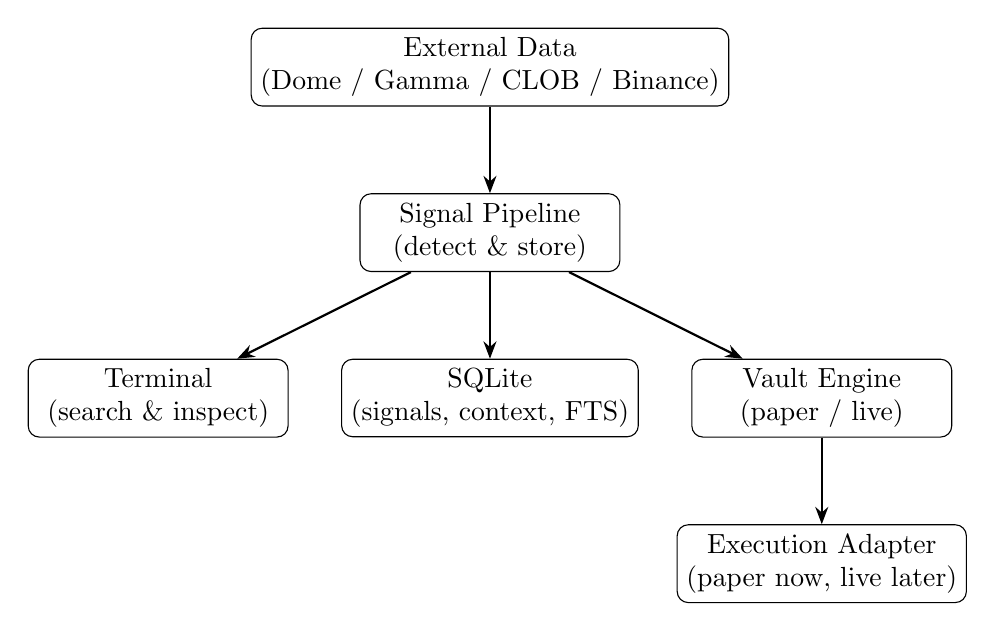
\begin{tikzpicture}[
  box/.style={rectangle, draw, rounded corners, minimum width=3.3cm, minimum height=0.9cm, align=center},
  arrow/.style={-{Stealth[length=2.2mm]}, thick},
]
\node[box] (sources) {External Data\\(Dome / Gamma / CLOB / Binance)};
\node[box, below=1.1cm of sources] (signals) {Signal Pipeline\\(detect \& store)};
\node[box, below left=1.1cm and 0.9cm of signals] (terminal) {Terminal\\(search \& inspect)};
\node[box, below right=1.1cm and 0.9cm of signals] (vault) {Vault Engine\\(paper / live)};
\node[box, below=1.1cm of vault] (exec) {Execution Adapter\\(paper now, live later)};
\node[box, below=1.1cm of signals] (db) {SQLite\\(signals, context, FTS)};

\draw[arrow] (sources) -- (signals);
\draw[arrow] (signals) -- (db);
\draw[arrow] (signals) -- (terminal);
\draw[arrow] (signals) -- (vault);
\draw[arrow] (vault) -- (exec);
\end{tikzpicture}
\caption{BETTER system flow: ingestion $\rightarrow$ signals $\rightarrow$ terminal/vault.}
\end{figure}

\section{Core implementation choices}
\begin{itemize}
  \item \textbf{Rust backend (Axum + Tokio):} high-concurrency API and background jobs.
  \item \textbf{SQLite (WAL mode):} durable, low-ops storage supporting 10M+ signals.
  \item \textbf{React 18 + TypeScript + Zustand:} terminal UI with merge-by-id hydration (REST + WS).
\end{itemize}

\clearpage

% =============================================================================
\chapter{Signal Pipeline}
% =============================================================================

\section{Data sources}
The implemented pipeline supports:
\begin{itemize}
  \item DomeAPI WebSocket for real-time wallet order events.
  \item DomeAPI REST for fallback polling and enrichment.
  \item Polymarket Gamma for market metadata.
  \item Polymarket CLOB book snapshots (token-id resolved and cached).
  \item Binance price feed for 15m Up/Down probabilistic evaluation.
\end{itemize}

\section{Signal types and storage}
Signals are stored as immutable primary records (id + type + details + timestamp) with optional context blobs attached asynchronously. The storage schema also maintains a full-history search index (FTS5) so the terminal can search beyond the currently loaded window.

\section{Search: ``never dead'' UX}
The terminal uses a server-backed full-history search endpoint when available, and falls back to local search over the loaded window when the search schema is not ready or the backend is unavailable. This prevents ``blank search'' regressions and preserves operator ergonomics.

\clearpage

% =============================================================================
\chapter{Execution and Vaults}
% =============================================================================

\section{Paper-first execution}
In this repository, order execution is modeled by a \emph{paper execution adapter} that simulates latency, slippage, fees, partial fills, and rejection. This enables end-to-end system validation (signal $\rightarrow$ decision $\rightarrow$ ledger) without live venue risk.

\section{Pooled vault accounting}
The pooled vault uses share-based NAV accounting:
\begin{itemize}
  \item Deposits mint shares at current NAV/share.
  \item Withdrawals burn shares and return USDC (cash-only withdrawals; liquidation not yet implemented).
\end{itemize}

\section{Mirror Vault upgrade path}
The Mirror Vault separates where capital resides (Base feeder vault) from where liquidity/composability is best (a Polygon-side ``master'' vault minting a receipt token such as \tokenvbetter{}). Receipt tokens can make strategy exposure transferrable and potentially tradable 24/7.

\section{Bounded agents and admissibility}
For non-deterministic decisions, \BETTER{} employs bounded agent outputs (admissible DSL records) and consensus gating (e.g., scout-first + 3-of-4 agreement). Malformed outputs abstain; risk caps and budgets bound compute and exposure.

\clearpage

% =============================================================================
\chapter{Risk Management}
% =============================================================================

\section{Principles}
Risk is managed by combining (i) conservative sizing, (ii) liquidity-aware constraints, (iii) throttles and cooldowns, and (iv) explicit budgets.

\section{Fractional Kelly sizing}
For a binary contract with implied market probability $p_m$ and an internal estimate $p_e$, an ``edge'' is $e = p_e - p_m$. A fractional Kelly sizing scheme is used with caps and guardrails.

\section{Guardrails (implemented patterns)}
\begin{itemize}
  \item Max position fraction of bankroll (per strategy).
  \item Min notional thresholds to avoid dust.
  \item Cooldowns to prevent churn.
  \item LLM budgets: max calls/day, max calls/market/day, and max tokens/day.
\end{itemize}

\clearpage

% =============================================================================
\chapter{Token Model and Economics (Proposed)}
% =============================================================================

\section{Utility: access and alignment}
\tokenbetter{} is designed as a utility/access key for terminal and vault participation. Gating reduces dilution of edge and aligns token demand with product demand.

\section{Fees (target model)}
\begin{itemize}
  \item \textbf{Vault fees:} performance fee on profits only, assessed on withdrawal.
  \item \textbf{Optional execution-path fee:} if an external execution router is used, a nominal trade fee may apply.
\end{itemize}

\section{Tokenomics (draft)}
\begin{table}[h]
\centering
\begin{tabular}{@{}lrrl@{}}
\toprule
\textbf{Allocation} & \textbf{\%} & \textbf{Tokens} & \textbf{Notes}\\
\midrule
Public sale (launchpad) & 25\% & 250,000,000 & Unlocked at TGE\\
Liquidity (Base/USDC LP) & 15\% & 150,000,000 & Locked permanently\\
Team & 20\% & 200,000,000 & Cliff + linear vesting (proposal)\\
Treasury & 25\% & 250,000,000 & Ops + strategic grants (proposal)\\
OpenServ drop & 5\% & 50,000,000 & Unlocked (proposal)\\
Programmatic funding & 10\% & 100,000,000 & Sold across FDV bands (proposal)\\
\bottomrule
\end{tabular}
\caption{Draft token allocation for \tokenbetter{} (subject to change).}
\end{table}

\section{Access gate (draft schedule)}
Access thresholds are intended to ratchet down as FDV increases to keep dollar-denominated access relatively stable and reward early holders.

\begin{table}[h]
\centering
\begin{tabular}{@{}llll@{}}
\toprule
\textbf{Phase} & \textbf{FDV band} & \textbf{Gate (\tokenbetter{})} & \textbf{Illustrative cost}\\
\midrule
1 & \textless{}\$10M & 100,000 & \$500--\$1,000\\
2 & \$10M--\$20M & 75,000 & \textasciitilde{}\$1,500\\
3 & \$20M--\$40M & 50,000 & \textasciitilde{}\$2,000\\
4 & \textgreater{}\$100M & 10,000 & \textasciitilde{}\$1,000\\
\bottomrule
\end{tabular}
\caption{Illustrative access-gate ratchet (draft; check app for current rules).}
\end{table}

\clearpage

% =============================================================================
\chapter{Roadmap (Indicative)}
% =============================================================================

\section{Phase 1: Tokenize the vault (Q1 2026)}
\begin{itemize}
  \item Token-gated terminal; stake-to-enable vault deposits.
  \item Productionize vault accounting, telemetry, and safety controls.
  \item Expand signal sourcing and operators.
\end{itemize}

\section{Phase 2: Arbitrage flywheel (Q2 2026)}
\begin{itemize}
  \item Receipt-token liquidity (\tokenvbetter{}) and LP incentives.
  \item Capture premium/discount dislocations to fund buy/burn (subject to execution reality).
\end{itemize}

\section{Phase 3: Performance markets / HIP-3 (Q4 2026)}
\begin{itemize}
  \item Long-horizon goal: performance-linked markets enabling hedging/leverage.
  \item Requires track record, backing, and strong risk constraints.
\end{itemize}

\clearpage

% =============================================================================
\chapter{Technical Annex (Reference Implementation)}
% =============================================================================

This annex includes curated excerpts from the repository to make the design auditable. Line ranges are pinned to the current code state and may drift as the code evolves.

\section{Backend: application state and router (Rust)}
\lstset{style=rust}
\maybeinputlisting[firstline=170,lastline=320]{../rust-backend/src/main.rs}
\maybeinputlisting[firstline=520,lastline=705]{../rust-backend/src/main.rs}

\clearpage
\section{Backend: API handlers (signals, search, vault)}
\maybeinputlisting[firstline=980,lastline=1450]{../rust-backend/src/api/simple.rs}

\clearpage
\section{Backend: SQLite schema + FTS5 search}
\lstset{style=rust}
\maybeinputlisting[firstline=1,lastline=360]{../rust-backend/src/signals/db_storage.rs}

\clearpage
\section{Backend: vault engine configuration + budgets}
\maybeinputlisting[firstline=30,lastline=240]{../rust-backend/src/vault/engine.rs}
\maybeinputlisting[firstline=540,lastline=660]{../rust-backend/src/vault/engine.rs}

\clearpage
\section{Backend: pooled vault (shares, deposit, withdraw)}
\maybeinputlisting[firstline=1,lastline=289]{../rust-backend/src/vault/pool.rs}

\clearpage
\section{Backend: execution adapters (paper + live placeholder)}
\maybeinputlisting[firstline=1,lastline=254]{../rust-backend/src/vault/execution.rs}

\clearpage
\section{Frontend: REST API client (TypeScript)}
\lstset{style=ts}
\maybeinputlisting[firstline=1,lastline=260]{../frontend/src/services/api.ts}
\maybeinputlisting[firstline=300,lastline=470]{../frontend/src/services/api.ts}

\clearpage
\section{Frontend: signal feed (search + local fallback)}
\maybeinputlisting[firstline=1,lastline=260]{../frontend/src/components/terminal/SignalFeed.tsx}
\maybeinputlisting[firstline=240,lastline=520]{../frontend/src/components/terminal/SignalFeed.tsx}

\clearpage

% =============================================================================
\chapter{Glossary}
% =============================================================================

\begin{description}[leftmargin=2.2cm,style=nextline]
  \item[Prediction market] A market where contracts settle on objective outcomes.
  \item[CLOB] Central Limit Order Book: bids/asks matched by price-time priority.
  \item[Alpha decay] The reduction of exploitable edge as information is priced in.
  \item[Vault] A pooled account where execution occurs on behalf of depositors.
  \item[Mirror vault] A feeder/master split: capital on one chain, receipts on another.
  \item[Receipt token] An ERC-20 representing a share of vault performance (e.g., \tokenvbetter{}).
  \item[Admissibility] A bounded set of outputs that are safe to execute; malformed outputs abstain.
\end{description}

\end{document}
